% L'option handout permet de supprimer la barre de navigation
\documentclass[handout]{beamer}
\usepackage[utf8]{inputenc}
\usepackage[french]{babel}
\usepackage[T1]{fontenc}
\usepackage{amsmath}
% Pour pouvoir insérer des images
\usepackage{graphicx}
\usepackage{wrapfig}
\graphicspath{images/}
% Gestion des couleurs
\usepackage{color}
\definecolor{turquoise}{RGB}{26, 188, 156}

% Un joli thème flat
\usetheme{Rochester}

% Personnalisation du thème
\usecolortheme[named=turquoise]{structure}
% Numéro de slides dans le footer
\setbeamertemplate{footline}[frame number]
\setbeamertemplate{blocks}[shadow=false]

\setbeamertemplate{footline}
{
	\leavevmode%
	\hbox{%
	\begin{beamercolorbox}[wd=.333333\paperwidth,ht=2.25ex,dp=1ex,center]{author in head/foot}%
		\usebeamerfont{author in head/foot}\insertsection
	\end{beamercolorbox}%
	\begin{beamercolorbox}[wd=.333333\paperwidth,ht=2.25ex,dp=1ex,center]{title in head/foot}%
		\usebeamerfont{title in head/foot}\insertsubsection
	\end{beamercolorbox}%
	\begin{beamercolorbox}[wd=.333333\paperwidth,ht=2.25ex,dp=1ex,right]{date in head/foot}%
		\usebeamerfont{date in head/foot}\insertshortdate{}\hspace*{2em}
		\insertframenumber{} / \inserttotalframenumber\hspace*{2ex}
	\end{beamercolorbox}}%
	\vskip0pt%
}

% ------------------------------------ %
% -- METADONNÉES DU DOCUMENT --------- %
\title{
	Projet Informatique Répartie - Diplo
}
\author{
	\textsc{Ansart}, \textsc{Augusti}, \textsc{Bernard},
	\textsc{Batise}, \textsc{Dauce}, \textsc{Malo}
}
\date{12 mai 2015}

% Début du document
\begin{document}

	% Génération de la page de titre
	\begin{frame}[plain]
		\titlepage
	\end{frame}

	% Génération du sommaire
	\begin{frame}[plain]
		\frametitle{Sommaire}
		\tableofcontents
	\end{frame}

	\section{Choix techniques}
		\subsection{Serveur}
	\begin{frame}
		\frametitle{API REST}
		\begin{itemize}
			\item Une API respectant les bonnes pratiques REST et HTTP;
			\item Entièrement en JSON;
			\item Une documentation claire et complète (\url{https://developers.diplo-lejeu.fr});
			\item Organisation en trois ressources : Conversations, Ordres, Parties;
			\item Documentation écrite en Markdown puis affichée sur une interface web.
		\end{itemize}
	\end{frame}

	\begin{frame}
		\frametitle{Composants}
		\begin{itemize}
			\item Framework MVC PHP : Laravel 5;
			\item ORM : Eloquent, intégré à Laravel;
			\item Base de données relationnelle : SQLite;
			\item Push / Pull Queue : IronMQ via \texttt{iron.io};
			\item Agrégateur d'exceptions : Bugsnag.
		\end{itemize}\bigskip
		Le tout hébergé sur un VPS chez RunAbove, à Roubaix. DNS et certificats SSL gérés par CloudFlare
	\end{frame}

	\begin{frame}
		\frametitle{Patterns utilisés}
		\begin{itemize}
			\item \textit{Repository pattern} : abstraction de l'accès au stockage;
			\item \textit{Middleware pattern} : pour les requêtes HTTP entrantes et la gestion des exceptions;
			\item \textit{Dependency injection} : injection automatique de classes concrètes implémentant des interfaces;
			\item Conception SOLID : beaucoup de classes spécialisées, contrôleurs HTTP de moins de 10 lignes.
		\end{itemize}
	\end{frame}

\subsection{Client}
	\begin{frame}
		\frametitle{Client}
	\end{frame}


	\section{Problèmes rencontrés}
		\subsection{Serveur}
	\begin{frame}
		\frametitle{Serveur}
        \begin{itemize}
            \item Reconception globale du programme; \newline
            \item Rédaction des spécifications de l'API; \newline
            \item Manque de tests complets. \newline
        \end{itemize}
	\end{frame}

\subsection{Client}
	\begin{frame}
		\frametitle{Client}
		\begin{itemize}
			\item Affichage de la carte; \newline
			\item Requête HTTPS - User Agent.
		\end{itemize}
	\end{frame}
	\begin{frame}[fragile]
		\frametitle{User-Agent}
		\begin{verbatim}
			Diplo/1.0

			Mozilla/5.0 (X11; Linux x86_64) 
			AppleWebKit/537.36 (KHTML, like Gecko) 
			Ubuntu Chromium/41.0.2272.76 
			Chrome/41.0.2272.76 
			Safari/537.36
		\end{verbatim}
	\end{frame}


	\section{Améliorations possibles}
		\subsection{Serveur}
	\begin{frame}
		\frametitle{Sécurité de l'application}
		\begin{itemize}
			\item Sécurité par l'IP ;
			\item Session ;
			\item Jeton d'authentification ;
			\item Authentification par compte utilisateur avec OAuth2.
		\end{itemize}
	\end{frame}

	\begin{frame}
		\frametitle{Protocole OAuth2}
		\begin{figure}[H]
			\centering
			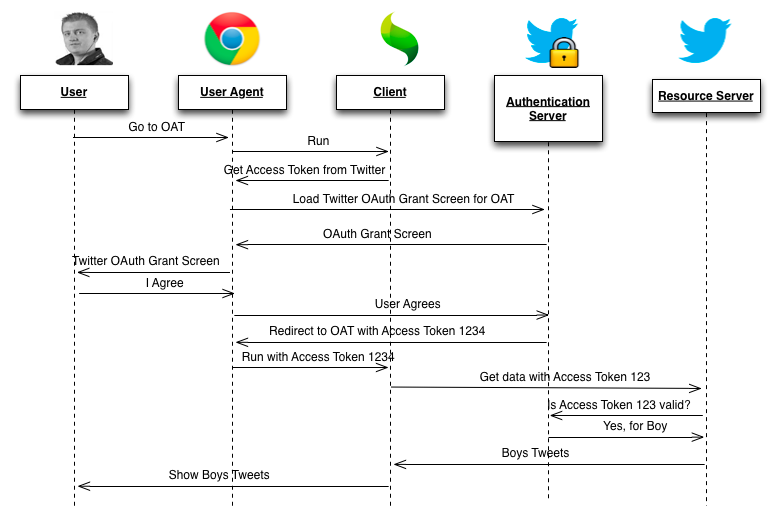
\includegraphics[scale=0.3]{images/oauth2.png}
			\caption{http://www.ibuildings.nl/blog/2013/03/secure-your-rest-api-oauth2-implicit-grant}
		\end{figure}

	\end{frame}

	\begin{frame}
		\frametitle{Autres améliorations}
		\begin{itemize}
			\item Performances :
				\begin{itemize}
					\item Amélioration des requêtes SQL ;
					\item Déléguer les requêtes à la base de données (fonction SQL) ;
					\item Changer de type de base de données (Neo4j ou PostgreSQL).
				\end{itemize}
			\item Séparation des services :
				\begin{itemize}
					\item Machines physiques ;
					\item Machines virtuelles.
				\end{itemize}
			\item Fonctionnalités :
				\begin{itemize}
					\item Cases maritimes ;
					\item Proposition de parties.
				\end{itemize}
		\end{itemize}
	\end{frame}

\subsection{Client}
	\begin{frame}
		\frametitle{Client}
		\begin{itemize}
			\item Amélioration de l'interface graphique ;
			\item Carte plus générique ;
			\item Refactor de la communication avec l'API ;
			\item Sérialisation / désérialisation des modèles grâce au JSON.
		\end{itemize}
	\end{frame}



\end{document}
